% Fachvortrag - Evolutionsstrategien - Jannis Weber + Niklas Hartinger - Praktikum Künstliche Intelligenz
\documentclass[%
	BCOR=8.25mm,         % Bindekorrektur
	DIV=12,              % Satzspiegel
	parskip=half,				 % Abstand zwischen Absätzen
	bibliography=totoc,	 % Literaturverzeichnis im Inhaltsverzeichnis
	headsepline=on,      % Trennlinie Kolumnentitel
	cleardoublepage=plain % page numbers on standard cleared double pages
	]{scrartcl}

%% Präambel
\usepackage[english, ngerman]{babel} % deutsche typogr. Regeln + Trenntabelle
\usepackage[T1]{fontenc}             % interner TeX-Font-Codierung
\usepackage{lmodern}                 % Font Latin Modern
\usepackage[utf8]{inputenc}          % Font-Codierung der Eingabedatei
\usepackage[babel]{csquotes}         % Anführungszeichen
\usepackage{graphicx}                % Graphiken
\usepackage{booktabs}                % Tabellen schöner
\usepackage{listingsutf8}            % Listings mit Einstellungen
\lstset{basicstyle=\small\ttfamily,
	tabsize=2,
	basewidth={0.5em,0.45em},
	extendedchars=true}
\usepackage{amsmath}	               % Mathematik
\usepackage[pdftex]{hyperref}
\hypersetup{
	bookmarksopen=true,
	bookmarksopenlevel=3,
	colorlinks=true,
	citecolor=black,
	linkcolor=black,
	urlcolor=magenta
}
\usepackage{scrhack}								 % unterdrückt Fehlermeldung von listings

%% Verzeichnisse
\usepackage{tocstyle} 
\usetocstyle{KOMAlike}

%% Nummerierungstiefen
\setcounter{tocdepth}{3}             % 3 Stufen im Inhaltsverzeichnis
\setcounter{secnumdepth}{3} 		     % 3 Stufen in Abschnittnummerierung




% CUSTOM ADDED PACKAGES START HERE

\usepackage{float}
\usepackage{caption}
\usepackage{subcaption}
%\usepackage[automake, acronym]{glossaries}
\usepackage{tabulary}
\usepackage{tikz}
\usepackage{listings}
\usepackage{color}
\usepackage{pdflscape}
\usepackage{tocloft}
\usepackage{amssymb}
\usepackage{xurl}

\usepackage[nottoc]{tocbibind}

% use equal fonts
\usepackage[scaled=.92]{helvet}
\usepackage{fancyhdr}

% fixes capitalization of header of bibliography
\fancypagestyle{bibliography}{%
  \renewcommand{\headrulewidth}{0.4pt}% reset to original width
  \fancyhf{}%
  \fancyhead[LE]{\fontfamily{ptm}\fontseries{m}\slshape\fontsize{11}{14}\selectfont Literaturverzeichnis}%
  \fancyhead[RO]{\fontfamily{ptm}\fontseries{m}\slshape\fontsize{11}{14}\selectfont Literaturverzeichnis}%
  \fancyfoot[LE]{\thepage}%
  \fancyfoot[RO]{\thepage}%
}

% keep page numbers for zusammenfassung, eidesstattliche erklärung und sperrvermerk
\fancypagestyle{entrypage}{%
  \renewcommand{\headrulewidth}{0pt}%
  \fancyhf{}%
  \fancyfoot[CE]{\thepage}%
  \fancyfoot[CO]{\thepage}%
}

\fancypagestyle{finalpage}{%
  \renewcommand{\headrulewidth}{0.4pt}% reset to original width
  \renewcommand{\headwidth}{30cm}% reset to original width
  \fancyhf{}%
  \fancyfoot[LE]{\hfill\hfill\thepage}%
  \fancyfoot[RO]{\hfill\hfill\thepage}%
}

% remove footnote counter reset after every section
%\counterwithout{footnote}{section}

\usepackage[hyperpageref]{backref}
\renewcommand*{\backref}[1]{}
\renewcommand*{\backrefalt}[4]{%
    \ifcase #1 [nicht zitiert]%
    \or        [zitiert auf Seite~#2]%
    \else      [zitiert auf Seite~#2]%
    \fi}
\backrefgerman

%\makeglossaries
%\loadglsentries{glossary}
%\loadglsentries{acronyms}

\lstset{literate=%
{Ö}{{\"O}}1
{Ä}{{\"A}}1
{Ü}{{\"U}}1
{ß}{{\ss}}2
{ü}{{\"u}}1
{ä}{{\"a}}1
{ö}{{\"o}}1
}

% fix old fonts
\makeatletter
\DeclareOldFontCommand{\rm}{\normalfont\rmfamily}{\mathrm}
\DeclareOldFontCommand{\sf}{\normalfont\sffamily}{\mathsf}
\DeclareOldFontCommand{\tt}{\normalfont\ttfamily}{\mathtt}
\DeclareOldFontCommand{\bf}{\normalfont\bfseries}{\mathbf}
\DeclareOldFontCommand{\it}{\normalfont\itshape}{\mathit}
\DeclareOldFontCommand{\sl}{\normalfont\slshape}{\@nomath\sl}
\DeclareOldFontCommand{\sc}{\normalfont\scshape}{\@nomath\sc}
\makeatother

% removes indentation of paragraphs at the start of a paragraph
\setlength{\parindent}{0pt}
% removes automatic spacing between paragraphs if page is not filled
\raggedbottom

%%% % Hurenkinder und Schusterjungen verhindern
%%% \clubpenalty = 10000 % schliesst Schusterjungen aus 
%%% \widowpenalty = 10000 \displaywidowpenalty = 10000 % schliesst Hurenkinder aus
%%% \widowpenalties=3 10000 10000 10000
% Hyphenpenalty
%%% %\usepackage[none]{hyphenat}
%%% %\righthyphenmin 10000
%%% %\hyphenchar\font=-1
\tolerance=1
\emergencystretch=\maxdimen
\hyphenpenalty=10000
\hbadness=10000

\usepackage{float}

\lstset{literate=%
{Ö}{{\"O}}1
{Ä}{{\"A}}1
{Ü}{{\"U}}1
{ß}{{\ss}}2
{ü}{{\"u}}1
{ä}{{\"a}}1
{ö}{{\"o}}1
}

\definecolor{lightgray}{rgb}{.9,.9,.9}
\definecolor{darkgray}{rgb}{.4,.4,.4}
\definecolor{purple}{rgb}{0.65, 0.12, 0.82}
\definecolor{darkgreen}{rgb}{0,.4,0}

\lstdefinelanguage{TypeScript}{
  keywords={await, typeof, new, true, false, catch, function, return, null, catch, switch, var, const, let, if, in, while, do, else, case, break, async, static},
  keywordstyle=\color{blue}\bfseries,
  ndkeywords={class, export, throw, implements, import, this},
  ndkeywordstyle=\color{darkgray}\bfseries,
  identifierstyle=\color{black},
  sensitive=false,
  comment=[l]{//},
  morecomment=[s]{/*}{*/},
  commentstyle=\color{purple}\ttfamily,
  stringstyle=\color{red}\ttfamily,
  morestring=[b]',
  morestring=[b]"
}

\newcommand{\setlistingtotypescript}[0]{
\lstset{
   language=TypeScript,
   backgroundcolor=\color{lightgray},
   extendedchars=true,
   basicstyle=\ttfamily\large,
   showstringspaces=false,
   showspaces=false,
   numbers=left,
   numberstyle=\footnotesize,
   numbersep=9pt,
   tabsize=2,
   breaklines=true,
   showtabs=false,
   captionpos=b,
   classoffset=1,
   sensitive=true,
   morekeywords={boolean, Boolean, number, Number, string, ITransportProfile, RoutingProfile, BuildingSetup, ILocation, Region, ICompound, PartialRoute, IPath, ORSResult, IPathResult},
   keywordstyle=\color{darkgreen},
   escapeinside=\$\$
}
}

\newcommand{\setlistingtocpp}[0]{
\lstset{
	language=C++,
	backgroundcolor=\color{lightgray},
	extendedchars=true,
	basicstyle=\ttfamily\large,
	showstringspaces=false,
	showspaces=false,
	numbers=left,
	numberstyle=\footnotesize,
	numbersep=9pt,
	tabsize=2,
	breaklines=true,
	showtabs=false,
	captionpos=b,
    keywordstyle=\color{blue},
	escapeinside=\$\$
}
}

\newcommand{\setlistingtosql}[0]{
\lstset{
	language=SQL,
	backgroundcolor=\color{lightgray},
	extendedchars=true,
	basicstyle=\ttfamily\large,
	showstringspaces=false,
	showspaces=false,
	numbers=left,
	numberstyle=\footnotesize,
	numbersep=9pt,
	tabsize=2,
	breaklines=true,
	showtabs=false,
	captionpos=b,
	morekeywords={int, varchar, double, tinyint, bigint, unsigned, REFERENCES, ENGINE, CHARSET, COMMENT},
	keywordstyle=\color{blue},
	escapeinside=\$\$,
}
}

\newcommand{\setlistingtopseudocode}[0]{
\lstset{
  	backgroundcolor=\color{lightgray},
  	extendedchars=true,
   	basicstyle=\ttfamily\large,
   	showstringspaces=false,
   	showspaces=false,
   	numbers=left,
   	numberstyle=\footnotesize,
   	numbersep=9pt,
   	tabsize=4,
   	breaklines=true,
   	showtabs=false,
   	captionpos=b,
   	classoffset=1,
   	sensitive=true,
   	mathescape=true
}
}

% for repeating a figure without being included in the list of figures
\newcommand{\repeatcaption}[2]{%
  \renewcommand{\thefigure}{\ref{#1}}%
  \captionsetup{list=no}%
  \caption{#2 (von Seite \pageref{#1})}%
  \addtocounter{figure}{-1}
}

% define fix usage of \Leftrightarrow, use as \noleftright
\newcommand{\notleftright}{\mathrel{\ooalign{$\Leftrightarrow$\cr\hidewidth$/$\hidewidth}}}

\DeclareCaptionType{equ}[][]
\makeatletter
\def\l@lstlisting#1#2{\@dottedtocline{1}{1.5em}{3em}{#1}{#2}}
\makeatother

% pulls section start upwards
%\RedeclareSectionCommand[beforeskip=0pt, afterskip=0.5cm]{section}

% see: https://tex.stackexchange.com/questions/161327/how-to-flip-even-odd-page-style
\let\tempmargin\oddsidemargin
\let\oddsidemargin\evensidemargin
\let\evensidemargin\tempmargin
\reversemarginpar

%--- ---%
% use \raggedbottom or \vfill to correct text placement if text was moved weirdly
%--- ---%

% ----------------------------------------------------------------------------
\begin{document}

\pagenumbering{Roman}

%% Titelseite
\begin{titlepage}
	\begin{center}
	
\includegraphics[width=0.9\textwidth]{img/mni-logo}
	
	\vspace{3cm}	

	\Large\textbf{\sffamily Ausarbeitung Fachvortrag}

	\vspace{1cm}	

	\huge\textbf{\sffamily Evolutionsstrategien}

	\normalsize
	\vspace{1cm}

	von \\[1cm]	

	\LARGE\textbf{Jannis Weber}\\ [.5cm]\normalsize
	Matrikelnummer: 5204678\\ [.75cm]
	
	\LARGE\textbf{Niklas Hartinger}\\ [.5cm]\normalsize
	Matrikelnummer: 5183113\\ [.75cm]
	
	im Dezember 2020
	\end{center}
	\vfill
	\begin{tabular}{ll}
		Dozent: & Professor Dr. Wolfgang Henrich 
	\end{tabular}
\end{titlepage}

%% Zusammenfassung
\pagestyle{entrypage}
% reset page to 1
\setcounter{page}{1}
\begin{quote}
	\vspace*{4cm}

	\begin{center}
		\textbf{\Large\sffamily Zusammenfassung}
	\end{center}
	\vspace*{.5cm}
	
\end{quote}

	Hier steht die Kurzzusammenfassung in deutsch.
	
\phantomsection
\addcontentsline{toc}{section}{Zusammenfassung}
\cleardoublepage

%% Verzeichnissse
%\settocfeature{entryhook}{\sffamily}    % alle Einträge wie im Text serifenlos
\tableofcontents
\cleardoublepage

\settocfeature{entryhook}{\rmfamily}    % Einträge wie im Text mit Serifen

\listoffigures
% durch \usepackage[nottoc]{tocbibind} nicht mehr notwendig
%\phantomsection
%\addcontentsline{toc}{section}{\listfigurename}
\cleardoublepage

\listoftables
% durch \usepackage[nottoc]{tocbibind} nicht mehr notwendig
%\phantomsection
%\addcontentsline{toc}{section}{\listtablename}
\cleardoublepage

\renewcommand\lstlistingname{Code-Listing}
\renewcommand\lstlistlistingname{Code-Listings}
\lstlistoflistings
\phantomsection
\addcontentsline{toc}{section}{\lstlistlistingname}
\cleardoublepage

\newcommand{\listequationsname}{Formelsammlung}
\newlistof{myequations}{equ}{\listequationsname}
\newcommand{\myequations}[1]{%
	\addcontentsline{equ}{section}{\protect\numberline{\theequation}#1}\par
}
\listofmyequations
\phantomsection
\addcontentsline{toc}{section}{\listequationsname}
\cleardoublepage

% Abstand im Inhaltsverzeichnis
\addtocontents{toc}{\vspace{\normalbaselineskip}}

\cleardoublepage

\pagenumbering{arabic}

% KAPITEL HIER EINFÜGEN
%-- einleitung

\section{Einleitung}

\subsection{Allgemeine Thematik}

In dieser Ausarbeitung werden die wesentlichen Evolutionsstrategien thematisiert.
Dabei handelt es sich um eine Kategorie der evolutionären Algorithmen, die sich seit den 1960er Jahren parallel zu den genetischen Algorithmen entwickelt hat.
Evolutionsstrategien\footnote{\textit{kurz:} ES} stellen wesentliche Modelle der Evolution für Computersimulationen und Anwendungen in der Informatik dar.
Ingo Rechenberg und Hans-Paul Schwefel sind schöpfende Persönlichkeiten, die die Evolutionsstrategien prägten und daraufhin die Rechenberg-Schwefel-Notation zur Modellierung von Evolutionsvorgängen durchsetzten.

Dieses Thema befasst sich mit allgegenwärtigen Optimierungsproblemen, die unter anderem auch technische Anwendung finden.
Bereits 1964 hat Rechenberg an der Universität Berlin mit der einfachsten Form der Evolutionsstrategien eine optimale Einstellung von Gelenkwinkeln einer Gelenkplatte berechnet \cite{schoeneburg}.
Ein weiteres Beispiel für ein kombinatorisches Optimierungsproblem ist das Problem des Handlungsreisenden (\textit{engl.} \enquote{traveling salesman problem}), dessen Bearbeitung im Anschluss an dieser fachlichen Ausarbeitung in einer gesonderten Ausarbeitung im Detail betrachtet wird.

In Abbildung \ref{fig:lokale_globale_maxima} sind die Auswirkungen der Wertfestlegung einzelner Parameter bei einem Optimierungsproblem beispielhaft zu sehen.
Unterschiedliche Kombinationen resultieren in unterschiedlich qualitativen Problemlösungen.
Um gewisse Parametereinstellungen befinden sich lokale Maxima, welche die nächstbeste Lösung im Vergleich zur aktuellen Parameterwahl darstellen. Diese bieten jedoch nur suboptimale Lösungen. Die optimale Lösung wird mit dem finden des globalen Qualitätsmaximum erreicht.

\begin{figure}[H]
\centering
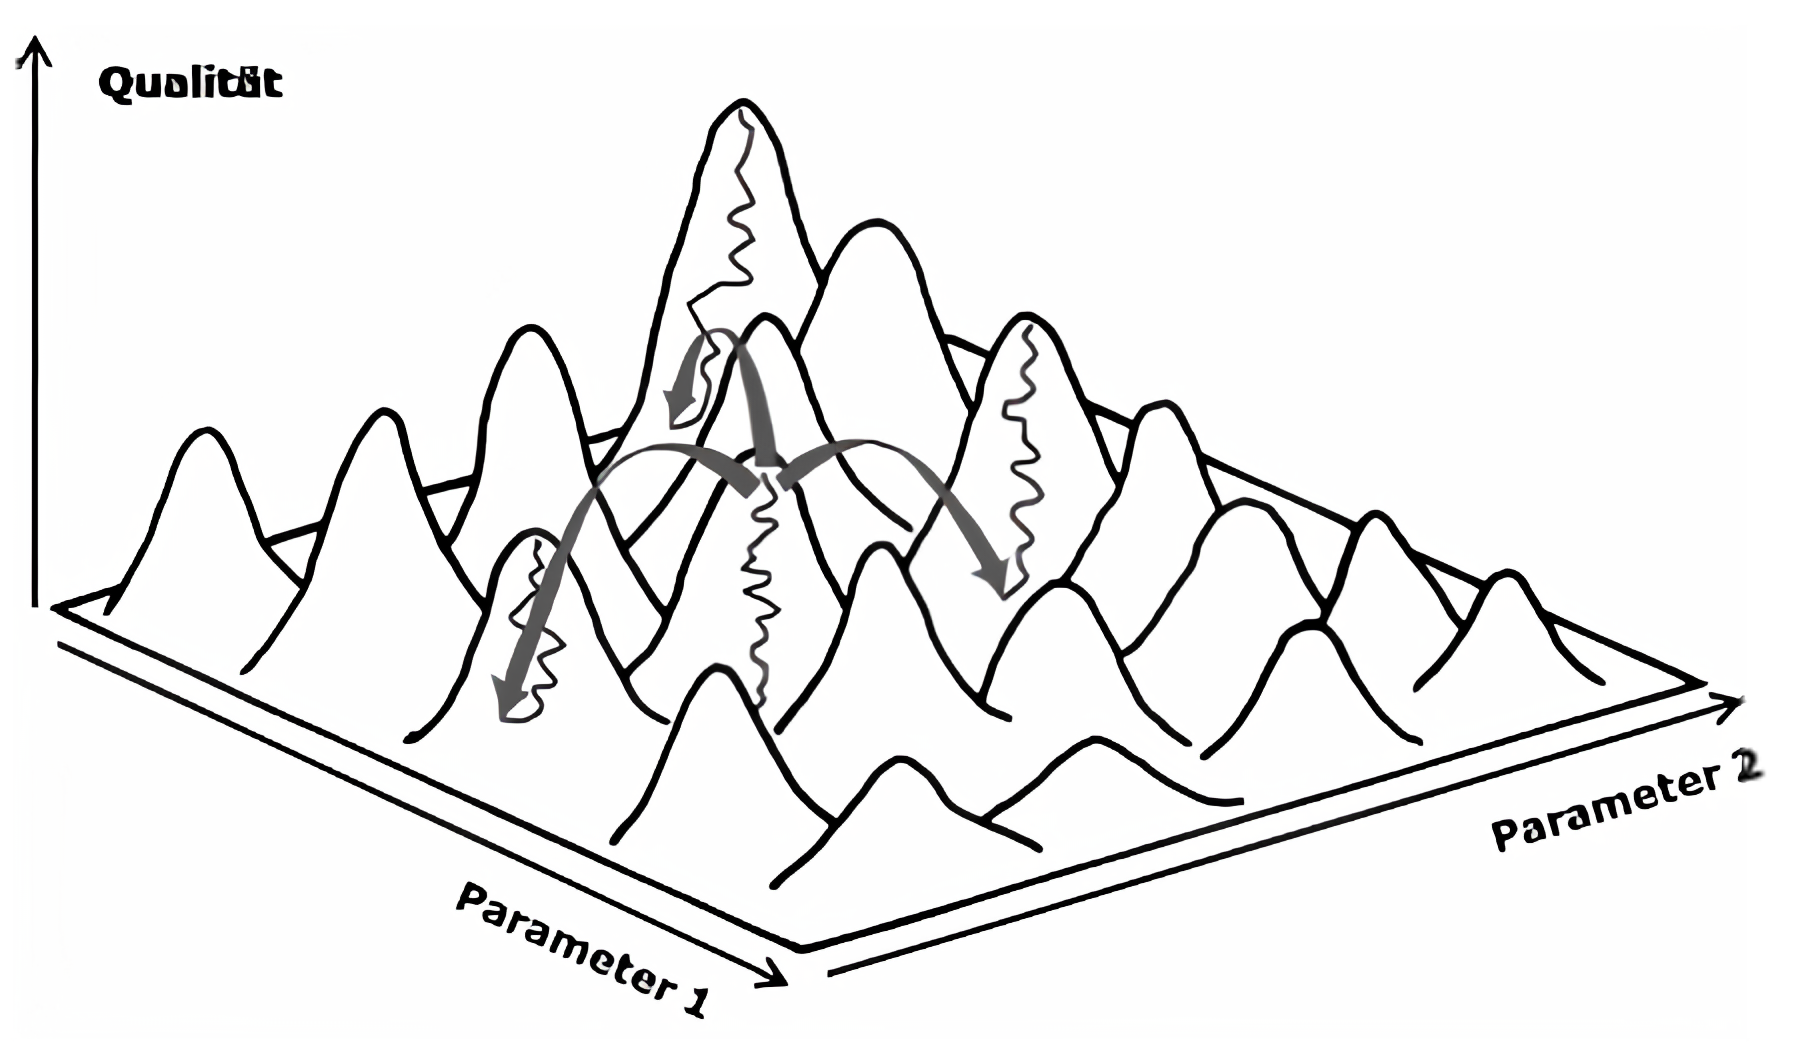
\includegraphics[width=0.65\textwidth]{img/Evolutionsstrategie_lokale_globale_Maxima.png}
\caption[Optimierungsprobleme: lokale Maxima/Minima finden]{Optimierungsprobleme: globales Qualitätsmaximum finden\protect\footnotemark}
\label{fig:lokale_globale_maxima}
\end{figure}
\footnotetext{\url{http://www.bionikvitrine.de/mediapool/99/996537/resources/17835925.png}}

Die Grundidee von evolutionären Algorithmen ist es nun, iterativ eine besser werdende Lösung eines Problems heranwachsen zu lassen.
Die Biologie dient dabei als Ansatzpunkt zur Modellierung einer möglichst stetigen Weiterentwicklung.
Nach dem Grundprinzip \enquote{survival of the fittest} soll sich die Lösung eines Optimierungsproblems über mehrere Generationen hinweg nach und nach in kleinen Anpassungsschritten dem Optimum annähern, bis eine nützliche Konfiguration von Parametern verwendet werden kann.

Abbildung \ref{fig:ablauf_einer_evolution} stellt die allgemeinen Evolutionsschritte sowie deren Ablauf dar.
Algorithmen zur Umsetzung einer speziellen Evolutionsstrategie unterscheiden sich an den Methodiken der Evolutionsschritte (\textit{siehe} Pfeilbeschriftungen).

\begin{figure}[H]
\centering
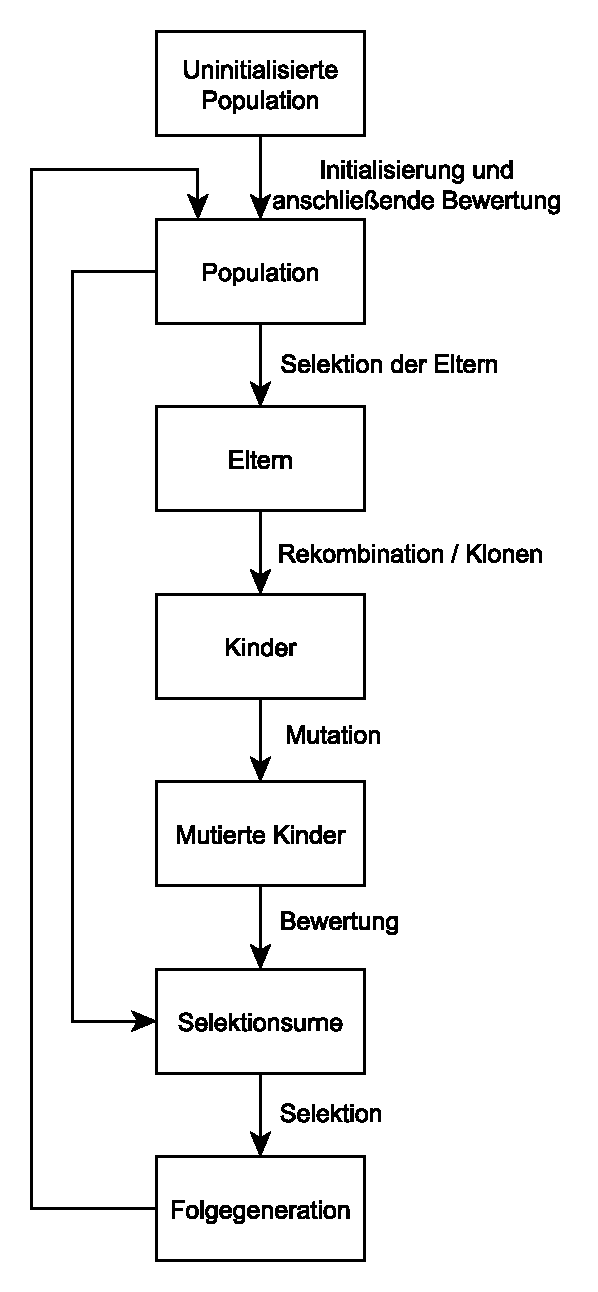
\includegraphics[width=0.4\textwidth]{img/ablauf_einer_evolution.pdf}
\caption[Ablauf einer Evolution]{Ablauf einer Evolution\protect\footnotemark}
\label{fig:ablauf_einer_evolution}
\end{figure}
\footnotetext{\url{http://www.evocomp.de/themen/evolutionsalgorithmen/pic/Evolutionsalgorithmen_Ablauf.gif}}

\pagebreak

Zu Beginn werden Parameterkonfigurationen, sogenannte \enquote{Individuen}, zufällig aufgebaut.
Anschließend werden daraus Eltern nach einem festgelegten Verfahren bestimmt, deren Informationen nach einem Klonvorgang bzw. einer Rekombination mehrerer Eltern an Kinder weitergegeben werden.
Zu einer gewissen Wahrscheinlichkeit werden die nachkommenden Individuen mutiert, bevor sie abschließend anhand einer Qualitätsfunkton nach deren \enquote{Fitness} für die nächste Generation selektiert werden.
Die qualitativ hochwertigsten Nachkommen dienen in der nächsten Iteration als Eltern.
Werden mehrere Individuen über den evolutionären Prozess hinweg beibehalten, spricht man bei einer Sammlung von Individuen von einer \enquote{Population}.

Eine Evolutionsstrategie gewährleistet keinen stetigen Qualitätsfortschritt. Oftmals kann eine Population an einem lokalen Maximum, als an einer suboptimalen Lösung, festhängen. Rückschritte in der Entwicklung sind auch möglich und hängen auch von der gewählten \enquote{Schrittweite} ab. Diese bestimmt, in welchem Maß die Parameterwerte eines von mindestens einem Elter stammenden Nachkommens angepasst werden.

\subsection{Aufbau der Ausarbeitung}

Nachdem die allgemeine Thematik im Grundsatz bekannt ist, wird im nächsten Abschnitt auf die Kodierung der Individuen eingegangen. Anschließend werden grundlegende, unterschiedliche Evolutionsstrategien behandelt, wobei jeweils ein zugehöriger Pseudocode-Abschnitt zur schnellen Umsetzung der jeweiligen Strategie dienen soll.

Dabei werden die Unterschiede zwischen den Evolutionsstrategien angesprochen. Hauptmerkmal der Evolutionsstrategien ist die Evolution. In Hinblick darauf wird die $\frac{1}{5}$-Regel als Grundtechnik und die mutative Schrittweitensteuerung zur Anpassung der Evolution detailliert aufgefasst.

%--
\section{Codierung}
% Was ist eine Codierung
Unter der Codierung eines Individuums versteht man eine Informationskette, die die relevanten Erbinformationen enthält.
% Codierung in der Natur
Die Gene eines Menschen können so als dessen Codierung angesehen werden.
% Codierung bei den Evolutionsstrategien
Bei den Evolutionsstrategien wurde auf eine komplizierte Codierung verzichtet und dafür eine sehr kure Codierungsform eingesetzt \cite[S.147]{schoeneburg}. Die relevanten Erbinformationen von Individuen werden durch Vektoren reeller Zahlen dargestellt \cite[S.147]{schoeneburg}. Diese Vektoren werden Chromosome genannt. Jedes Individuum hat ein solches Chromosom.
Eine Menge an Individuen bildet eine Population. Diese Codierungsweise wird in der Grafik \ref{fig:codierung} dargestellt. Darin ist zu sehen, wie eine Menge an Individuuen eine Population bildet. Die Individuen sind als Männchen verbildlicht. Darüber hinaus ist ein Chromosomausschnitt zu sehen.\\
Die Wahl für diese Codierungsvariante lässt sich darauf zurückführen, dass die Evolutionsstrategien zu Beginn für ingenieurstechnische Optimierungen verwendet wurden \cite[S.147]{schoeneburg}.
In diesem Aufgabenfeld werden optimale Systemparameter gesucht. Diese lassen sich sehr gut als Vektoren reeler Zahlen abbilden.\\
Der durch die Evolutionsstrategien gewählte Codierungansatz wird als phänotypisch orientiert bezeichnet \cite[S.148]{schoeneburg}. Das bedeutet, dass im Gegensatz zu einer genotypischen Orientierung, die Eigenschaft des Individuums betrachtet wird , die sich aus den Chromosomen ergeben, und nicht die Chromosome selbst.
Die Eigenschaft des Individuums kann durch Qualitätsfunktionen berechnet werden.

\begin{figure}[!htb]
	\centering
	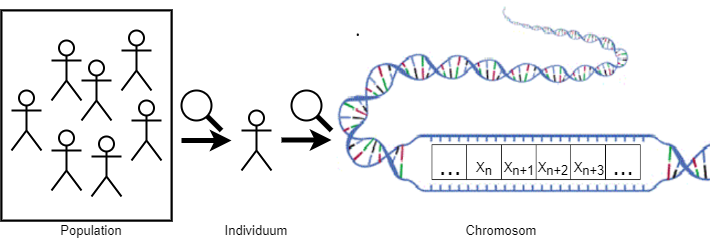
\includegraphics[width=1.\textwidth]{img/codierung/codierung.png}
	\caption{Grafische Darstellung einer Population, von Individuen und eines Chromosoms.}
\label{fig:codierung}
\end{figure}



\section{Typisches Aussehen einer Evolutionsstrategie}
%1. Obwohl viel Variation, erkannte Rechenberg Abschnitte die häufig wiederzufinden sind
Evolutionsstrategien weisen einen sehr hohen Grad an variation auf. Je nach Aufgabengebiet können sich die Verfahren stark unterscheiden.
Rechenberg konnte allerdings Verfahrensabschnitte benennen, welche aus denen sich typischerweise Evolutionsstrategien zusammensetzen.
Diese Verfahrensabschnitte bilden die Rechenbergsche Grafik-Notation. Diese Notation orientiert sich an Spielkarten und kommt mit lediglich 10 verschiedenen Symbolen aus.
Die Komplexität der Evolutionsstrategien wird durch deren Kombination erreicht.
%2. Die Rechenbergnotation erklären

%individuum
\begin{figure}[!htb]
	\centering
	
\includegraphics[scale=0.5]{img/rechenberg_notation/individuum.png}
	\caption{Individuum}
\label{fig:individuum}
\end{figure}
%population
\begin{figure}[!htb]
	\centering
	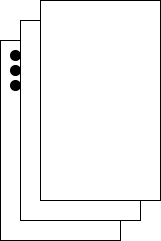
\includegraphics[scale=0.5]{img/rechenberg_notation/population.png}
	\caption{Population}
\label{fig:population}
\end{figure}
%population isoliert
\begin{figure}[!htb]
	\centering
	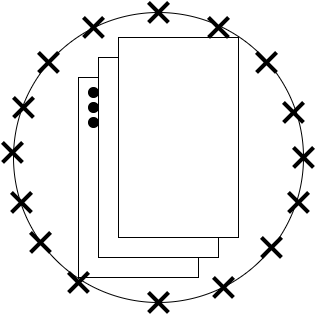
\includegraphics[scale=0.5]{img/rechenberg_notation/population_isoliert.png}
	\caption{Isolierte Population}
\label{fig:population_isoliert}
\end{figure}
%auswahl
\begin{figure}[!htb]
	\centering
	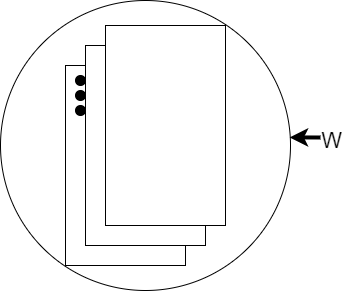
\includegraphics[scale=0.5]{img/rechenberg_notation/auswahl_gleichverteilt.png}
	\caption{Gleichverteilte Auswahl}
\label{fig:auswahl_gleichverteilt}
\end{figure}
\begin{figure}[!htb]
	\centering
	\includegraphics[scale=0.5]{img/rechenberg_notation/auswahl_qualitätsfunktion.png}
	\caption{Auswahl mit einer Qualitätsfunktion}
\label{fig:auswahl_qualitätsfunktion}
\end{figure}
%duplikation
\begin{figure}[!htb]
	\centering
	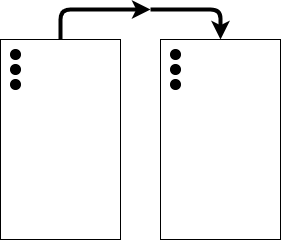
\includegraphics[scale=0.5]{img/rechenberg_notation/duplikation.png}
	\caption{Duplikation}
\label{fig:duplikation}
\end{figure}
%mutation
\begin{figure}[!htb]
	\centering
	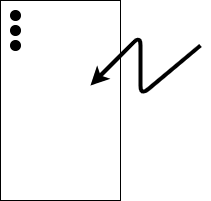
\includegraphics[scale=0.5]{img/rechenberg_notation/mutation.png}
	\caption{Mutation}
\label{fig:mutation}
\end{figure}
%bewertung
\begin{figure}[!htb]
	\centering
	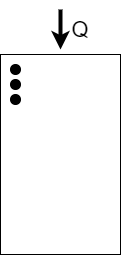
\includegraphics[scale=0.5]{img/rechenberg_notation/bewertung.png}
	\caption{Bewertung}
\label{fig:bewertung}
\end{figure}
%rekombination
\begin{figure}[!htb]
	\centering
	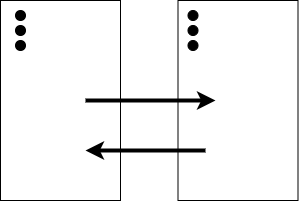
\includegraphics[scale=0.5]{img/rechenberg_notation/rekombination.png}
	\caption{Rekombination}
\label{fig:rekombination}
\end{figure}
%phänotypische realisierung
\begin{figure}[!htb]
	\centering
	\includegraphics[scale=0.5]{img/rechenberg_notation/phänotypische_realisation.png}
	\caption{Phänotypische Realisation}
\label{fig:phänotypische_realisation}
\end{figure}


% 3. Typische Reihenfolge der Abschnitte kurz zeigen. Aber auch klar machen das das ganze extrem variieren kann

%-- steuerung der evolution

\section{Steuerung der Evolution}

\subsection{$(1+1)$-ES}

Die $(1+1)$-Evolutionsstrategie gilt als einfachste Form der ES. Mit ihr hat Rechenberg 1964 die optimale Einstellung von Gelenkwinkeln einer Gelenkplatte berechnen lassen.

Es handelt sich um eine zweigliedrige Strategie, bei dem es in jeder Evolutionsiteration genau ein Ur-Individuum bzw. Elternindividuum gibt, welches der Erzeugung von genau einem nachkommenden Individuum (Kindindividuum) dient. Dabei wird der Ausgangsvektor analog zum biologischen Prozess der DNS-Selbstverdopplung dupliziert. Das zweite, bislang wertgleiche, Individuum wird anschließend zufällig, allerdings nicht willkürlich modifiziert. Meist wird ein kleiner reeller Wert auf jeden Vektorparameter addiert.

Die beiden, nun unterschiedlichen, Individuen werden nach dem Prinzip \enquote{survival of the fittest} bewertet.
Anhand des Outputs einer Qualitätsfunktion wird verglichen, welcher der beiden Individuen das zielführendere ist und anschließend zur Fortführung der Evolution selektiert werden soll.
Umgangssprachlich spricht man von einem \enquote{Sterben der Schwachen} und einem \enquote{Überleben der Starken}.
Bei gleicher Qualitätsbewertung wird ein Individuum zufällig selektiert.
Als Zeitmaß für die Evolutionsiteration dient die \enquote{Generation}, wobei die Generation $G_0$ die Ausgangsgeneration mit einem Ausgangsindividuum bildet. Die Selektion aus dessen Elterindividuum sowie dessen Nachkomme bildet die Generation $G_1$ und so weiter.

Aus diesem Vorgehen bedeutet die Namensgebung "$(1+1)$-ES": Ein Elternindividuum wird zusammen mit einem nachkommenden Individuum für die Selektion betrachtet.

In diesem Fall wird das Erbgut ausschließlich über die Mutation verändert. Es gibt keine sexuelle Rekombination des Erbgutes.

Es handelt sich zwar um eine grundlegende und kompakte Form der Abbildung von Evolutionsmechanismen, jedoch entsteht auch hierbei in Kombination mit der adaptiven Schrittweitenregelung zur Mutation der Nachkommen (\textit{siehe Kapitel \ref{sec:mutation}}) sinnvolle Anwendungen.

\begin{lstlisting}[caption={$(1+1)$-Evolutionsstrategie}\label{lst:1_und_1_es}, firstnumber=1, captionpos=b, label=code:1_und_1_es]
<@\colorcodeline{algorithm baue\_individuum(n)}@>
	individuum <- []	
	for _ <- 1...n
		individuum <- individuum + zufälliges $x \in \mathbb{R}$
	return individuum
	
<@\colorcodeline{algorithm qualitaet(individuum | population}@>
	// problemspezifische Qualitätsfunktion

	
<@\colorcodeline{algorithm duplikation(individuum[1...n])}@>
	klon <- []
	for i <- 1...n
		klon <- klon + individuum[i]
	return klon
	
<@\colorcodeline{algorithm selektion(individuen[1...m]), $\mu$, qualitaetsfunktion}@>
	sortierteIndividuen <- sortiereAbsteigend(individuen, qualitaetsfunktion)
	besteIndividuen <- []
	for i <- 1,...,$\mu$
		besteIndividuen <- besteIndividuen + sortierteIndividuen[i]
	return besteIndividuen
	

<@\colorcodealgorithm{algorithm $(1+1)$-ES()}@>
	iterationsLimit <- x $\in \mathbb{N}$
	generationszaehler <- 0
	wunschqualitaet <- y $\in \mathbb{R}$
	individuengroesse <- n $\in \mathbb{N}$
	<@\colorcodeline{individuum <- baue\_individuum(individuengroesse)}@>
	while qualitaet(individuum) < wunschqualitaet and generationszaehler < iterationslimit:
		generationszaehler <- generationszaehler + 1
		elter <- individuum
		<@\colorcodeline{kind <- duplikation(elter)}@>
		kind <- mutation(kind)
		individuum <- selektion([elter, kind], 1, qualitaet)
	loesung <- individuum
\end{lstlisting}

\subsection{$(\mu + \lambda)$-ES}

Mit der $(\mu + \lambda)$-Evolutionsstrategie wird die vorige $(1+1)$-ES in einer allgemeineren Form übertragen.
Dabei gilt:
\begin{equation}
|Nachkommen| \ge |Eltern| \ge 1 \Leftrightarrow \lambda \ge \mu \ge 1
\end{equation}
Es müssen aus den $\mu$ Eltern also $\lambda$ viele Nachkommen erzeugt werden, wobei es mehr Nachkommen als Eltern geben muss.
Alle Individuen werden gemeinsam für eine Selektion der besten Individuen betrachtet.
Somit können einige Elternindividuen über mehrere Generationen hinweg bestehen, sofern sie sich einem im Vergleich hohen Fitnesswert zuordnen lassen.

Das \enquote{+} der $(\mu + \lambda)$-Notation lässt sich somit als Vereinigung sowohl der Eltern als auch der Nachkommen lesen, die abschließend gemeinsam selektiert werden.

Werden mehrere Nachkommen erzeugt als es Eltern gibt, also:
\begin{equation}
|Nachkommen| > |Eltern| \Leftrightarrow \lambda > \mu
\end{equation}
dann müssen einige Eltern mehrfach zur Erzeugung eines Nachkommens ausgewählt werden.
Von allen Individuen werden anschließend die $|Eltern| = \mu$ besten ausgewählt. Die Größe der Elternpopulation bleibt somit immer konstant. Da die Eltern \textbf{und} die Nachkommen bewertet werden und zur Selektion bereitstehen, wird die Qualität des Besten der nächsten Population niemals schlechter als die der vorigen.

Algorithmisch sind die Anzahlen der Nachkommen und der Eltern folglich nun frei wählbar, wobei die Anzahl der zu erzeugenden Nachkommen mindestens so groß wie die Anzahl der Elternindividuen sein muss.

\begin{lstlisting}[caption={$(\mu + \lambda)$-Evolutionsstrategie}\label{lst:mu_und_lambda_es}, firstnumber=1, captionpos=b, label=code:mu_und_lambda_es]
<@\colorcodeline{algorithm baue\_population($\mu$, n)}@>
	population <- []
	for i <- 1...$\mu$
		individuum <- baue_individuum(n)
		population <- population + individuum
	return population
	
<@\colorcodeline{algorithm elternSelektion(population[1,...,$\mu$], $\lambda$)}@>
	individuen <- []
	for _ <- 1...$\lambda$
		idx <- zufälliges x $\in {1,...,\mu}$
		individuum <- population[idx]
	return individuen
	

<@\colorcodeline{algorithm duplikation(individuen[1...$\mu$], n)}@>
	klone <- []
	for i <- 1...$\mu$
		klon <- []
		for j <- 1...n
			klon <- klon + individuen[i][j]
		klone <- klone + klon
	return klon
	
<@\colorcodeline{algorithm bestenSelektion(population[1,...,$\mu$])}@>
	beste_loesung <- []
	for i <- 1...$\mu$
		individuum <- population[i]
		if fitness(individuum) > fitness(beste_loesung)
			beste_loesung <- individuum
	return beste_loesung
	

<@\colorcodealgorithm{algorithm $(\mu + \lambda)$-ES()}@>
	iterationsLimit <- x $\in \mathbb{N}$
	generationszaehler <- 0
	anzahl_eltern <- $\mu \ge 1$
	anzahl_kinder <- $\lambda \ge$ anzahl_eltern
	wunschqualitaet <- y $\in \mathbb{R}$
	individuengroesse <- n $\in \mathbb{N}$
	population <- baue_population($\mu$, individuengroesse)
	while qualitaet(individuum) < wunschqualitaet and generationszaehler < iterationslimit:
		generationszaehler <- generationszaehler + 1
		<@\colorcodeline{eltern <- elternSelektion(population, anzahl\_kinder)}@>
		<@\colorcodeline{kinder <- duplikation(eltern, individuengroesse)}@>
		kinder <- mutation(kinder)
		<@\colorcodeline{population <- selektion(eltern + kinder, $\mu$, qualitaet)}@>
	loesung <- bestenSelektion(population)
\end{lstlisting}

\subsection{$(\mu, \lambda)$-ES}

Als weitere Evolutionsstrategie gibt es die Komma-Notation, welche von Schwefel in seiner Dissertation 1975 eingeführt wurde. Bei $(\mu + \lambda)$-ES kann das beste Individuum nicht vergessen gehen, da in jeder Iteration alle Individuen bei der Selektion berücksichtigt werden. Auf den ersten Blick klingt dies nach einem wünschenswerten Effekt, jedoch können negative Auswirkungen die Folge sein, wenn es sich dabei um ein lokales Optimum laut der Qualitätsfunktion handelt.
Das globale Optimum und somit die optimale Lösung des Problems wird daraufhin häufig nicht mehr gefunden.

Schwefels $(\mu, \lambda)$-ES nutzt einen veränderten Selektionsmechanismus:
Die Elternindividuen werden bei der abschließenden Selektion nicht mehr berücksichtigt und somit vergessen. Es werden lediglich $|Eltern| = \mu$ der $|Nachkommen| = \lambda$ Nachkommen für die nächste Generation ausgewählt.

Insofern handelt es sich um ein naturgetreues Modell der Evolution. Kein Individuum ist mehr unsterblich. Allerdings sterben sie direkt nach einer Generation. Aufgrund dessen sind allerdings auch Rückschritte in der Evolution möglich.

Generell werden geringfügige normalverteilte Mutationen bevorzugt, um nur leichte Veränderungen der Nachkommen hervorzurufen.

\begin{lstlisting}[caption={$(\mu, \lambda)$-Evolutionsstrategie}\label{lst:mu_nur_lambda_es}, firstnumber=1, captionpos=b, label=code:mu_nur_lambda_es]
<@\colorcodealgorithm{algorithm $(\mu , \lambda)$-ES()}@>
	iterationsLimit <- x $\in \mathbb{N}$
	generationszaehler <- 0
	anzahl_eltern <- $\mu \ge 1$
	anzahl_kinder <- $\lambda \ge$ anzahl_eltern
	wunschqualitaet <- y $\in \mathbb{R}$
	individuengroesse <- n $\in \mathbb{N}$
	population <- baue_population($\mu$, individuengroesse)
	while qualitaet(population) < wunschqualitaet and generationszaehler < iterationslimit:
		generationszaehler <- generationszaehler + 1
		eltern <- elternSelektion(population, anzahl_kinder)
		kinder <- duplikation(eltern, individuengroesse)
		kinder <- mutation(kinder)
		<@\colorcodeline{population <- selektion(kinder, $\mu$, qualitaet)}@>
	loesung <- bestenSelektion(population)
\end{lstlisting}

\subsection{$(\mu \# \lambda)$-ES}

Die $(\mu \# \lambda)$-Notation bedeutet lediglich, dass das Selektionsverfahren keine Rolle spielt.
Es werden aus den $\mu$ Eltern $\lambda$ Nachkommen erzeugt. Die Selektion kann beliebig durchgeführt werden.

\subsection{Selektionsdruck und Populationswellen}

$(\mu \# \lambda)$-ES erlauben eine einfache Beschreibung und Simulation des Selektionsdrucks innerhalb einer Population als auch von Populationswellen.
Bei dem Selektionsdruck handelt es sich um einen Quotienten $s = \frac{\mu}{\lambda}$, wobei $0 < s < 1$.
Er besagt, in welchem Verhältnis die Anzahl der Elternindividuen zu den Nachkommen stehen.
Je größer die Anzahl der erzeugten Nachkommen $\lambda$ im Verhältnis zu den Eltern $\mu$, desto mehr Individuen werden erzeugt, als in die nächste Generation übernommen werden können.
Liegt $\lambda$ dicht bei $\mu$, so werden nur wenige Individuen aufgrund einer schlechten Bewertung aussortiert und folglich nicht in die nächste Generation übernommen.
Somit steht $0$ für einen starken und $1$ für einen schwachen Selektionsdruck.

Unter Populationswellen versteht man eine Anpassung der Parameter $\mu$ und $\lambda$ einer Evolutionsstrategie über Generationen hinweg. Insofern dient eine unterschiedliche Anzahl an Eltern der Erzeugung einer unterschiedlichen Anzahl an Nachkommen.
Um einen gleichbleibenden Selektionsdruck zu erzielen, müssen die Parameter $\mu$ und $\lambda$ stets in gleichem Verhältnis zueinander stehen und können nur eingeschränkt angepasst werden.

In Bezug auf die Biologie sind periodisch und zyklische Variationen des Selektionsdrucks interessant.

\subsection{$(\mu / p \# \lambda)$-ES}

In den bislang genannten Evolutionsstrategien wurde die sexuelle Rekombination nicht berücksichtigt.
Diese wird mit der $(\mu / p \# \lambda)$-ES nun betrachtet.
In den Grundzügen baut diese Evolutionsstrategie auf den vorigen auf, jedoch gibt es nun einen Unterschied bei der Erzeugung von Duplikaten.
Anstatt einzelne Individuen werden nun Gruppen von Individuen herangezogen.
das $p$ entspricht somit der Anzahl der Elemente einer Gruppe zur Erzeugung eines Nachkommens.

Standardmäßig werden dazu zwei Eltern ($p = 2$) genutzt.
In diesem Fall wird an den einzelnen Vektorelementen per Zufall entschieden, ob eine Vertauschung der Werte durchgeführt wird.
Aus den beiden resultierenden Individuen wird per Zufall nur einer ausgewählt.

\begin{lstlisting}[caption={$(\mu / p \# \lambda)$-Evolutionsstrategie mit $p = 2$}\label{lst:mu_p2_lambda_es}, firstnumber=1, captionpos=b, label=code:mu_p2_lambda_es]
<@\colorcodeline{algorithm gruppenSelektion(population[1...$\mu$], $\lambda$, p)}@>
	gruppen <- []
	for i <- 1...$\lambda$
		gruppe <- []
		for j <- 1...p
			idx <- zufälliges $x \in {1,...,\mu}$
			individuum <- population[idx]
			gruppe <- gruppe + individuum
		gruppen <- gruppen + gruppe
	return gruppen

<@\colorcodeline{algorithm rekombination(gruppen[1,...,$\lambda$], p, n)}@>
	individuen <- []
	for i <- 1...$\lambda$
		individuum <- []
		gruppenindividuen <- gruppen[i]
		for j <- 1...n
			idx <- zufälliges $x \in {1,...,p}$
			gruppenindividuum <- gruppenindividuen[idx]
			individuum <- individuum + gruppenindividuum[j]
		individuen <- individuen + selectSingleBest(gruppenindividuen)
	return individuen

<@\colorcodealgorithm{algorithm $(\mu / p \# \lambda)$-ES()}@>
	iterationsLimit <- x $\in \mathbb{N}$
	generationszaehler <- 0
	anzahl_eltern <- $\mu \ge 1$
	anzahl_kinder <- $\lambda \ge$ anzahl_eltern
	wunschqualitaet <- y $\in \mathbb{R}$
	individuengroesse <- n $\in \mathbb{N}$
	population <- baue_population($\mu$)
	gruppengroesse <- $p = 2$
	while qualitaet(population) < wunschqualitaet and generationszaehler < iterationslimit:
		generationszaehler <- generationszaehler + 1
		<@\colorcodeline{eltern\_gruppen <- gruppenSelektion}@>(population, anzahl\_kinder, gruppengroesse)
		<@\colorcodeline{kinder <- rekombination}@>(eltern\_gruppen, gruppengroesse, individuengroesse)
		kinder <- mutation(kinder)
		population <- selektion(kinder, $\mu$, qualitaet) // oder selektion(eltern + kinder, $\mu$, qualitaet)
	loesung <- bestenSelektion(population)
\end{lstlisting}


Ist $p > 2$, so spricht man von einer Multirekombination.
Dabei werden die Mittelwerte der reellen Zahlen an den Positionen der zu rekombinierenden Vektoren und somit das nachkommende Individuum gebildet.

\begin{lstlisting}[caption={$(\mu / p \# \lambda)$-Evolutionsstrategie mit $p > 2$}\label{lst:mu_pgt2_lambda_es}, firstnumber=1, captionpos=b, label=code:mu_pgt2_lambda_es]
<@\colorcodeline{algorithm rekombination(gruppen[1,...,$\lambda$], p, n)}@>
	individuen <- []
	for i <- 1...$\lambda$
		individuum <- []
		gruppenindividuen <- gruppen[i]
		for j <- 1...n
			value <- 0
			for k <- 1...p
				gruppenindividuum <- gruppenindividuien[k]
				value <- value + gruppenindividuum[j]
			value <- value / p
			individuum <- individuum + value
		individuen <- individuen + individuum
	return individuen

<@\colorcodealgorithm{algorithm $(\mu / p \# \lambda)$-ES()}@>
	iterationsLimit <- x $\in \mathbb{N}$
	generationszaehler <- 0
	anzahl_eltern <- $\mu \ge 1$
	anzahl_kinder <- $\lambda \ge$ anzahl_eltern
	wunschqualitaet <- y $\in \mathbb{R}$
	individuengroesse <- n $\in \mathbb{N}$
	population <- baue_population($\mu$)
	gruppengroesse <- p $| p > 2$
	while qualitaet(population) < wunschqualitaet and generationszaehler < iterationslimit:
		generationszaehler <- generationszaehler + 1
		eltern_gruppen <- gruppenSelektion(population, anzahl_kinder, gruppengroesse)
		<@\colorcodeline{kinder <- rekombination}@>(eltern\_gruppen, gruppengroesse, individuengroesse)
		kinder <- mutation(kinder)
		population <- selektion(kinder, $\mu$, qualitaet) // oder selektion(eltern + kinder, $\mu$, qualitaet)
	loesung <- bestenSelektion(population)
\end{lstlisting}


\subsection{Populationen}

In den bislang erwähnten Evolutionsstrategien wurden lediglich einzelne Individuen erzeugt, mutiert und selektiert.
Nun sollen aber auch mehrere Populationen herangezogen werden.
Dafür ist eine besondere Notation notwendig.
Im Folgenden meinen runde Klammern weiterhin Individuen, während eckige Klammern die Populationen beschreiben.

Als Beispiel wird die $[6,9(2+4)]$-ES betrachtet:\\
Zuerst ist die eckige Klammer zu entziffern. Hier werden $\mu_p = 6$ unabhängige Populationen verwendet, um  $\lambda_p = 9$ Populationen zu erzeugen, wobei nur die erzeugten Populationen bei der Selektion betrachtet werden.\\
In jeder Population dienen (laut der inneren Klammer) $\mu_i = 2$ Elternindividuen zur Erzeugung von $\lambda_i = 4$ Nachkommen. Diese werden mit den Eltern zusammen zur Selektion betrachtet.

Eine Population wird auch nach ihrer Qualität bewertet.
Dazu kann beispielsweise die mittlere Qualität aller Individuen der Population dienen.
Eine Population kann alternativ nach der Qualität ihres besten Individuums bewertet werden, oder nach der Streuung der einzelnen Fitnesswerte der Individuen.

\begin{lstlisting}[caption={Evolutionsstrategien mit mehreren Populationen}\label{lst:populationen_es}, firstnumber=1, captionpos=b, label=code:populationen_es]
<@\colorcodeline{algorithm baue\_populationen(ps, $\mu$, n)}@>
	populationen <- []
	for i <- 1...ps
		population <- baue_population($\mu$, n)	
		populationen <- populationen + population
	return populationen
	
<@\colorcodeline{algorithm bestenSelektion(population[1,...,$\mu$])}@>
	beste_loesung <- []
	for i <- 1...$\mu$
		individuum <- population[i]
		if fitness(individuum) > fitness(beste_loesung)
			beste_loesung <- individuum
	return beste_loesung

<@\colorcodealgorithm{algorithm Populationen-ES()}@>
	iterationsLimit <- x $\in \mathbb{N}$
	generationszaehler <- 0
	anzahl_populationen <- y $| y \ge 2$
	anzahl_eltern <- $\mu \ge 1$
	anzahl_kinder <- $\lambda \ge$ anzahl_eltern
	wunschqualitaet <- y $\in \mathbb{R}$
	individuengroesse <- n $\in \mathbb{N}$
	<@\colorcodeline{populationen <- baue\_populationen(anzahl\_populationen, $\mu$)}@>
	while qualitaet(populationen) < wunschqualitaet and generationszaehler < iterationslimit:
		for i <- 1...anzahl_populationen
			generationszaehler <- generationszaehler + 1
			population <- populationen[i]
			eltern <- elternSelektion(population, anzahl_kinder)
			kinder <- duplikation(eltern, individuengroesse) // oder rekombination bei elterngruppen
			kinder <- mutation(kinder)
			population <- selektion(kinder, $\mu$, qualitaet) // oder selektion(eltern + kinder, $\mu$, qualitaet)
	<@\colorcodeline{loesung <- bestenSelektion(populationen)}@>
\end{lstlisting}

In der Notation kann auch das \enquote{Vermischungssymbol} \textbf{/} verwendet werden. Dadurch können einzelne Individuen zwischen den Populationen getauscht werden.

\begin{lstlisting}[caption={Evolutionsstrategien mit mehreren Populationen und Individuentausch}\label{lst:populationen_ind_vertauschen_es}, firstnumber=1, captionpos=b, label=code:populationen_ind_vertauschen_es]
<@\colorcodeline{algorithm tauscheIndividuen(populationen[1...y], )}@>
	// beliebiges Vertauschungsverfahren

<@\colorcodealgorithm{algorithm Population-ES()}@>
	iterationsLimit <- x $\in \mathbb{N}$
	generationszaehler <- 0
	anzahl_populationen <- y $| y \ge 2$
	anzahl_eltern <- $\mu \ge 1$
	anzahl_kinder <- $\lambda \ge$ anzahl_eltern
	wunschqualitaet <- y $\in \mathbb{R}$
	individuengroesse <- n $\in \mathbb{N}$
	populationen <- baue_populationen(anzahl_populationen, $\mu$)
	while qualitaet(populationen) < wunschqualitaet or generationszaehler < iterationslimit:
		for i <- 1...anzahl_populationen
			generationszaehler <- generationszaehler + 1
			population <- populationen[i]
			eltern <- elternSelektion(population, anzahl_kinder)
			kinder <- duplikation(eltern, individuengroesse) // oder rekombination bei elterngruppen
			kinder <- mutation(kinder)
			population <- selektion(kinder, $\mu$, qualitaet) // oder selektion(eltern + kinder, $\mu$, qualitaet)
		<@\colorcodeline{tauscheIndividuen(populationen)}@>
	loesung <- bestenSelektion(populationen)
\end{lstlisting}

\subsubsection{Isolierte Populationen}

Isolierte Populationen durchlaufen eine individuelle Entwicklung auf bestimmte Zeit.
Zur Zeitangabe wird in der Notation eine hochgestellte Isolationszahl verwendet, welche die Isolation einer Population meist in Anzahl Generationen angibt.

Es werden abgeschottete Entwicklungen abgebildet.
Nachdem eine isolierte Population erzeugt wird, durchläuft sie folglich eine eigene Entwicklung.
Erst danach steht sie der Selektion der besten Populationen zur Verfügung.

Isolierte Populationen ermöglichen eine hochgradige Parallelität der Suche im Suchraum des Optimierungsproblems.

\begin{lstlisting}[caption={Evolutionsstrategien mit isolierten Populationen}\label{lst:isolierte_populationen_es}, firstnumber=1, captionpos=b, label=code:isolierte_populationen_es]
<@\colorcodealgorithm{algorithm Isolierte-Populationen-ES()}@>
	iterationsLimit <- x $\in \mathbb{N}$
	isolationsiterationen <- z $| z \ge 2$
	generationszaehler <- 0
	anzahl_populationen <- y $| y \ge 2$
	anzahl_eltern <- $\mu \ge 1$
	anzahl_kinder <- $\lambda \ge$ anzahl_eltern
	wunschqualitaet <- y $\in \mathbb{R}$
	individuengroesse <- n $\in \mathbb{N}$
	populationen <- baue_populationen(anzahl_populationen, $\mu$)
	while qualitaet(populationen) < wunschqualitaet or generationszaehler < iterationslimit:
		generationszaehler <- generationszaehler + 1
		for i <- 1...anzahl_populationen
			population <- populationen[i]
			isolationzaehler <- 0			
			<@\colorcodeline{while isolationzaehler $\le$ isolationsiterationen}@>
				isolationzaehler <- isolationzaehler + 1
				eltern <- elternSelektion(population, anzahl_kinder)
				kinder <- duplikation(eltern) // oder rekombination bei elterngruppen
				kinder <- mutation(kinder)
				population <- selektion(kinder, $\mu$, qualitaet) // oder selektion(eltern + kinder, $\mu$, qualitaet)
	loesung <- bestenSelektion(populationen)
\end{lstlisting}

\subsection{Abbruchbedingungen}

Wird als Abbruchkriterium nicht die Qualität der Nachkommen zusammen in Betracht gezogen, so kann ein vorzeitiger Abbruch das Finden einer optimalen Lösung verhindern.
Dies ist beispielsweise bei dem Erreichen einer gewissen Generationszahl der Fall.

Beispiele für Abbruchkriterien der Durchführungsiterationen von ES:
\begin{itemize}
	\item Qualität der Nachkommen
	\item Rechenzeit
	\item Anzahl erzeugter Generationen
	\item ...
\end{itemize}

%-- Standard-Evolutionsstrategie

\section{Standard-Evolutionsstrategie}
Die bisherigen Kapitel haben gezeigt, dass eine Evolutionsstrategie beliebig kompliziert aufgebaut sein kann. Eine komplexere Evolutionsstrategie führt aber natürlich nicht automatisch zu besseren Ergebnissen \cite[S.~165]{schoeneburg}.
In diesem Kapitel wird die standardmäßige Komplexität erklärt. Anschließend werden die von Rechenberg definierten optimalen Parameter erläutert. Das Kapitel schließt mit dem Aufzeigen der Schwächen der Notation ab.

\subsection{Komplexität}
Obwohl dieses Kapitel Standard-Evolutionsstrategie heißt, gibt es keine vollumfängliche Strategie, die für alle Anwendungsgebiete eingesetzt werden kann. Viel mehr wird standardmäßig eine maximale Komplexität verwendet \cite[S.~165]{schoeneburg}.
Die Komplexität kann mit der Anzahl an Iterationsstufen gesteuert werden, denn in jeder Iterationsstufe können wiederum evolutionäre Vorgänge durchgeführt werden.
Für praktische Anwendungen macht es wenig Sinn eine zu große Iterationsstufe zu wählen \cite[S.~165]{schoeneburg}. Aus diesem Grund endet der standardmäßige Einsatz von Evolutionsstrategien mit der zweiten Iterationsstufe.
Somit ist die Evolutionsstrategie aus Formel \ref{eqn:standard_equation} die komplexeste Strategie die standardmäßig eingesetzt wird. Hierbei muss aber betont werden, dass \textit{standardmäßig} ein sehr schwammiger Begriff ist. 
Ob ein Anwendungsfall standardmäßig ist, müssen die Anwender eigenständig feststellen und in diesem Vorgang verschiedene Evolutionsstrategien testen. Es sollte dabei aber mit einer möglichst geringen Komplexität begonnen werden.

\begin{equation}
\label{eqn:standard_equation}
[u/v\,\#\,w (x/y\,\#\,z)^{/n}]-ES\, \cite[S.~165]{schoeneburg}
\end{equation}
\myequations{Standard-Evolutionsstrategie}

\subsection{Parameter}
Die verschiedenen Evolutionsstrategien setzen sich aus den Parametern $\lambda, \mu$ und $p$ zusammen. So ist dies beispielsweise der $(\mu / p \# \lambda)$-Evolutionsstrategie \ref{eqn:opt_parameter} zu entnehmen.

\begin{equation}
\label{eqn:opt_parameter}
(\mu/p\,\#\,\lambda)-ES
\end{equation}
\myequations{$(\mu / p \# \lambda)$-Evolutionsstrategie}

Genau wie es Richtwerte für die Komplexität einer Evolutionsstrategie gibt, so gibt es auch Richtwerte für die Wahl der Parameter \cite[S.~166]{schoeneburg}.
Der Quotient $\frac{\mu}{\lambda}$ gibt den Selektionsdruck der Strategie wieder. Dieser Selektionsdruck soll laut Rechenberg zwischen $\frac{1}{3}$ und $\frac{1}{5}$ liegen  \cite[S.~166]{schoeneburg}. Rechenberg empfiehlt bei einer einfachen, glatten Qualitätsfunktion zur Beurteilung einzelner Individuen den Selektionsdruck von $\frac{1}{5}$  \cite[S.~166]{schoeneburg}.
Der Parameter $p$ soll so gewählt werden, dass er maximal so groß wie $\mu$ ist \cite[S.~166]{schoeneburg}. Somit können Individuen auch mehr als zwei Eltern haben. Das erscheint aus der Natur vielleicht nicht normal, stellt in den Evolutionsstrategien allerdings kein Hindernis dar. Gilt $p = \mu$, so handelt es sich darüber hinaus um eine vollständige Multirekombination.
Bei der Konstruktion einer Evolutionsstrategie sollten die Anwender zu Beginn innerhalb der Richtwerte arbeiten, um zu untersuchen, ob mit diesen Parameterwerten schon ausreichend gute Ergebnisse erzielt werden können. Erst danach sollten komplexere Parametereinstellungen überprüft werden.
Rechenberg selbst liefert ein Beispiel, in dem die Regel nicht anzuwenden ist. Er empfiehlt bei einer mutativen Schrittweitenregelung eine Parameterwahl von $\mu = 1$ und $\lambda = 10$ \cite[S.~166]{schoeneburg}. Der so erzeugte Quotient liegt außerhalb der Richtlinie, soll in bestimmten Fällen aber trotzdem zu guten Ergebnissen führen.

\subsection{Uneindeutigkeiten der Notation}

Obwohl die Rechenberg-Schwefel'sche Notation bei der Konstruktion von Evolutionsstrategien stark unterstützt, gibt es Schwächen in der Notation, die den Anwender einschränken können.
Unter anderem kann nicht angegeben werden, welche Mutations- und Rekombinationsverfahren verwendet werden, weil diese Details hinter der Abstraktion verborgen bleiben.

Beispielsweise kommen bereits mit dem Vermischungssymbol \enquote{/} Fragen bezüglich des Rekombinationsverfahrens auf.
Soll eine gleichverteilte Zufallsauswahl stattfinden oder eine Parameterselektion durch die Mittelwertbildung?

Darüber hinaus ist es in der Notation nicht möglich darzustellen, dass sich Populationen simultan aber trotzdem unterschiedlich entwickeln sollen. So könnten zum Beispiel unterschiedliche Rekombinations- und Mutationsverfahren angewendet werden.
Die Schwächen der Notation sorgen also dafür, dass durch eine zu große Abstraktion wichtige Details verloren gehen. 
Daher empfiehlt es sich, die notwendigen Informationen anhand einer schriftlichen Dokumentation in Form von Text oder Pseudocode nachzuliefern.

%--- mutation

\section{Mutation}
\label{sec:mutation}

Das entscheidende Merkmal von Evolutionsstrategien ist der Fokus auf die Mutation.

Während die Selektion von Elternindividuen zur Erzeugung von Nachkommen und die evtl. durchgeführte Rekombination anhand der statistischen Gleichverteilung stattfinden, wird die Mutation nach der statistischen Normalverteilung vollzogen.

Statistische Gleichverteilung bedeutet, dass jedes Individuum bei der Selektion der Eltern mit der gleichen Wahrscheinlichkeit ausgewählt werden kann. Die Selektion ist somit unabhängig von der Qualität der Individuen. Dieses Verfahren wird auch bei der Selektion der Vektorwerte bei der Rekombination von zwei Elternindividuen verwendet.

Bei der Mutation hingegen kommt die Normalverteilung zum Einsatz. Dabei ist es wahrscheinlicher, dass eine Zufallsvariable seine Ausprägung nah am Erwartungswert hat. Werte, die weit vom Erwartungswert entfernt sind, sind relativ unwahrscheinlich, je nach Standardabweichung. Generell werden geringfügige, normalverteilte Mutationen bevorzugt, um nur leichte Veränderungen bei den Nachkommen hervorzurufen. Insofern ist die Normalverteilung sehr praktisch.

In den folgenden Kapiteln wird beschrieben, welchen Grundsatz diese Funktionsweise verfolgt und wie die Mutation im Pseudocode umgesetzt werden kann.
Zunächst werden die mathematischen Grundlagen der Normalverteilung kurz aufgegriffen.

\subsection{Normalverteilung}

Die Normal- bzw. Gauß-Verteilung ist ein wichtiger Typ stetiger Wahrscheinlichkeitsverteilungen.
Stetig bezieht sich in diesem Zusammenhang auf die Zufallsvariablen, die in einem beliebigen Intervall eine unendliche Menge an Werten annehmen können.
Als Gegenspieler gibt es diskrete Zufallsvariablen, die eine abzählbare Menge an Ausprägungen in einem Intervall darstellen.

Die wichtigen Kennwerte von Wahrscheinlichkeitsverteilungen sind \enquote{Mittelwert}, \enquote{Varianz} und \enquote{Standardabweichung} \cite[S.~168]{schoeneburg}.

Als Mittelwert $\mu$ wird das arithmetische Mittel aller möglichen Ausprägungen der Zufallsvariablen definiert. Dieses wird über die Summe aller Werte geteilt durch die Anzahl $n$ an Ausprägungen bestimmt:

\begin{equation}
\mu = \frac{1}{n} \sum_{i=1}^n a_i
\end{equation}
\myequations{Mittelwert $\mu$}

\pagebreak

Die Varianz sowie die Standardabweichung geben die Schwankung der Werte von dem Erwartungswert an.
Die Varianz $\sigma^2$ wird mit folgender Formel gebildet:

\begin{equation}
\sigma^2 = \frac{1}{n} \sum_{i=1}^n (a_i-\mu)^2
\end{equation}
\myequations{Varianz $\sigma^2$}

Die Standardabweichung $\sigma$ entspricht somit der Wurzel der Varianz:

\begin{equation}
\sigma = \sqrt{\sigma^2} = \sqrt{\frac{1}{n} \sum_{i=1}^n (a_i-\mu)^2}
\end{equation}
\myequations{Standardabweichung $\sigma$}

Die Normalverteilung wird anhand des Mittelwerts und der verwendeten Standardabweichung notiert:

\begin{equation}
N(\mu, \sigma)
\end{equation}
\myequations{Notation der Normalverteilung}

Die Verteilungsfunktion der Normalverteilung gibt an, zu welcher Wahrscheinlichkeit F(x) der Wert die Ausprägung $\le x$ ist. Sie ist gegeben durch:

\begin{equation}
F(x) = \frac{1}{\sqrt{2 \pi \sigma^2}} \int_{-\infty}^x e^{-\frac{(x-\mu)^2}{2 \sigma^2}} dx
\end{equation}
\myequations{Verteilungsfunktion}

Abbildung \ref{fig:verteilungskurven} stellt einige Verteilungsfunktionen beispielhaft dar.

\begin{figure}[H]
\centering
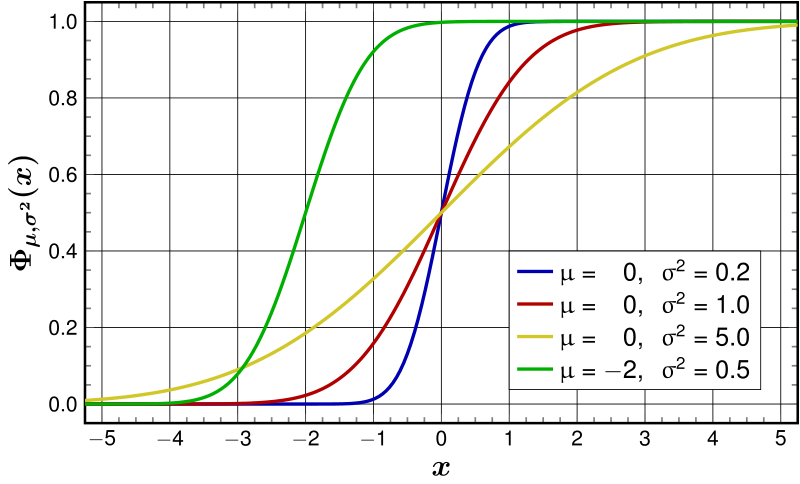
\includegraphics[width=0.75\textwidth]{img/Verteilungskurven.png}
\caption[Verteilungsfunktionen]{Verteilungsfunktionen\protect\footnotemark}
\label{fig:verteilungskurven}
\end{figure}
\footnotetext{\url{https://upload.wikimedia.org/wikipedia/commons/thumb/7/74/Normal-distribution-cumulative-density-function-many.svg/800px-Normal-distribution-cumulative-density-function-many.svg.png}}

Die Dichtefunktion bzw. die Wahrscheinlichkeitsdichte der Normalverteilung ergibt sich aus der Ableitung $F'(x)$ der Verteilungsfunktion $F(x)$ und ist eine Glockenkurve \cite[S.~172]{schoeneburg}:

\begin{equation}
f(x) = F'(x) = \frac{1}{\sqrt{2 \pi \sigma^2}} e^{-\frac{(x-\mu)^2}{2 \sigma^2}}
\end{equation}
\myequations{Dichtefunktion / Wahrscheinlichkeitsdichte}

Deren Streckung bzw. Stauchung lässt sich anhand der Standardabweichung einstellen. Die x-Achsenverschiebung wird durch den Erwartungswert vorgenommen\footnote{\textit{siehe} Tool zur Visualisierung: \url{https://www.geogebra.org/m/e2Ppkaj9}}. Abbildung \ref{fig:glockenkurven} veranschaulicht unterschiedliche Dichtefunktionen von Normalverteilungen.

\begin{figure}[H]
\centering
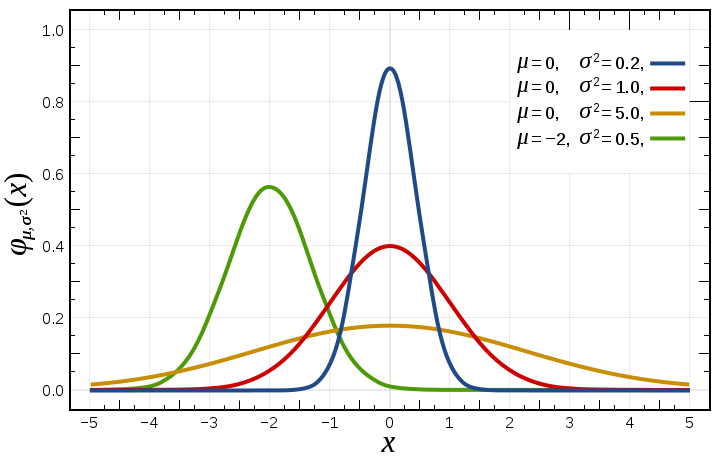
\includegraphics[width=0.75\textwidth]{img/Glockenkurven.png}
\caption[Dichtefunktionen]{Dichtefunktionen\protect\footnotemark}
\label{fig:glockenkurven}
\end{figure}
\footnotetext{\url{https://upload.wikimedia.org/wikipedia/commons/thumb/7/74/Normal_Distribution_PDF.svg/720px-Normal_Distribution_PDF.svg.png}}

Eine Teilfläche unterhalb der Dichtefunktion beschreibt die Wahrscheinlichkeit, dass eine Zufallsvariable eine Ausprägung in dem festgelegten Bereich annimmt. Sie wird errechnet durch die Formel:

\begin{equation}
P(x_1 \le X \le x_2) = \int_{x_1}^{x_2} f(x) dx
\end{equation}
\myequations{Wahrscheinlichkeit einer Ausprägung in einem Bereich}

\subsection{Standardnormalverteilung}

Jede Normalverteilung lässt sich mithilfe der folgenden Substitution $z = \frac{x - \mu}{\sigma}$ in die Standardnormalverteilung überführen:

\begin{equation}
z = \frac{x - \mu}{\sigma}
\end{equation}
\myequations{Substitution zur Überführung in die Normalverteilung}

\begin{equation}
P(X \le x) = \Phi(\frac{x - \mu}{\sigma}) = \Phi(z)
\end{equation}
\myequations{Ablesen der Wahrscheinlichkeit}

Da eine eigenhändige Berechnung ohne Hilfsmittel sehr aufwändig ist, wird dieser Trick angewendet, um die Wahrscheinlichkeiten anhand einer vorgefertigten Standardnormalverteilungstabelle abzulesen, wie in Abbildung \ref{fig:standardnormalverteilung} zu sehen.

\begin{figure}[H]
\centering
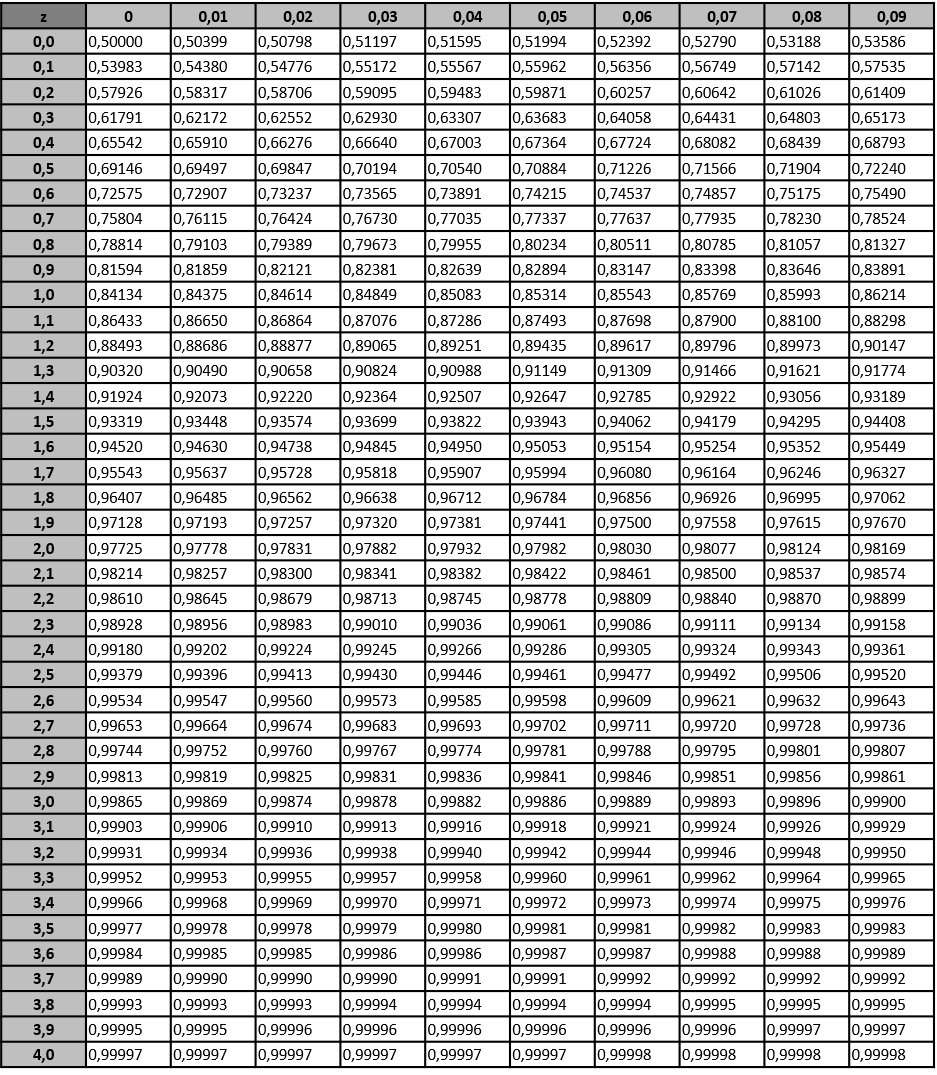
\includegraphics[width=\textwidth]{img/Standardnormalverteilung_Tabelle.png}
\caption{Wahrscheinlichkeitstabelle der Standardnormalverteilung}
\label{fig:standardnormalverteilung}
\end{figure}

\subsection{Mutative Schrittweitenregelung}

Die Idee der mutativen Schrittweitenregelung ist es nun, die reellen Vektorwerte eines Individuums bei der Mutation anhand von Zufallszahlen der $N(0, \sigma)$-Verteilung in jeder Generation anzupassen. Da der Mittelwert $0$ ist, werden hauptsächlich kleine Änderungen vorgenommen. Es gibt jedoch keine bestimmte Suchrichtung. Die Schrittweite der Mutation kann über die Standardabweichung konfiguriert werden. Es werden also positive und negative Zahlen auf die Vektorwerte addiert. Jeder Vektorwert wird um eine neue Zufallszahl aus dieser Verteilung verändert \cite[S.~174-175]{schoeneburg}.

\begin{equation}
x_{neu} = x_{alt} + N(0, \sigma)
\end{equation}
\myequations{Mutation eines Parameterwertes}

Nach einer analytischen Untersuchung von einfachen Qualitätsfunktionen zur Analyse der optimalen Streuung der Zufallszahlen ermittelte Rechenberg anhand des \enquote{Korridor}- und des \enquote{Sphären}-Modells, dass die optimale Streuung ungefähr $\frac{1}{5}$ beträgt. Insofern solle der Anteil an erfolgreichen Mutationen zur Verbesserung der Qualität des betroffenen Individuums über mehrere Generationen durchschnittlich mindestens $\frac{1}{5}$ betragen. Wird dieser Wert unterschritten, so wird die Streuung bzw. Standardabweichung erhöht. Wird er überschritten, wird die Streuung verringert.

Die Regeln der Anpassung der Schrittweite (Standardabweichung) je nach Erfolgs- bzw. Verbesserungsrate ergeben sich somit als \cite[S.~179]{schoeneburg}:

\begin{enumerate}
	\item $\sigma(x+n) = c \cdot \sigma(x)\ |\ p > \frac{1}{5}$
    \item $\sigma(x+n) = d \cdot \sigma(x)\ |\ p < \frac{1}{5}$
    \item $\sigma(x+n) = \sigma(x)\ |\ p = \frac{1}{5}$
\end{enumerate}
\myequations{$\frac{1}{5}$-Regel zur Schrittweitenanpassung}

Laut Schwefel empfiehlt es sich, $c = 1,22$ und $d = 0,82$ zu verwenden.

Durch die Anpassung der Schrittweite wird also je nach Anteil an erfolgreichen Mutationen die Standardabweichung angepasst, was dazu führt, dass die Zufallszahlen zur Mutation der Vektorwerte des Individuums je nach Veränderung noch wahrscheinlicher an $0$ bzw. etwas weiter entfernt von $0$ liegen und somit die Veränderung des gesamten Individuums in kleinerem bzw. größerem Maße geschieht.

Im Pseudocode \ref{lst:mutative_schrittweitenrgelung_es} sieht der Vorgang entsprechend so aus:

\begin{lstlisting}[caption={Mutative Schrittweitenregelung}, firstnumber=1, captionpos=b, label=lst:mutative_schrittweitenrgelung_es]
<@\colorcodeline{algorithm mutation(individuen[1,...,$\mu$], $\sigma$, n)}@>
	mutierteIndividuen <- []
	for i <- 1,...,$\mu$
		individuum <- individuen[i]
		mutiertesIndividuum <- [1,...,n]		
			for j <- 1,..,n
				z <- Zufallszahl $\in$ $N(0, \sigma)$
				mutiertesIndividuum[j] <- individuum[j] + z
		mutierteIndividuen <- mutierteIndividuen + mutiertesIndividuum
	return mutierteIndividuen
	
<@\colorcodeline{algorithm berechneAnteilVerbesserungen}@>(startIndividuen[1,...,$\mu$], mutierteIndividuen[1,...,$\mu$])
	verbesserungen <- 0	
	for i <- 1,...,$\mu$
		if qualitaet(mutierteIndividuen[i]) > qualitaet(startIndividuen[i])
			verbesserungen <- verbesserungen + 1
	return verbesserungen / $\mu$
	
<@\colorcodeline{algorithm passeStandardabweichungAn($\sigma$, p)}@>
	c <- 1.22
	d <- 0.82
	if p > $\frac{1}{5}$
		return c * $\sigma$
	else if p < $\frac{1}{5}$
		return d * $\sigma$
	else
		return $\sigma$

<@\colorcodealgorithm{algorithm Mutative-Schrittweitenregelung-ES()}@>
	iterationsLimit <- x $\in \mathbb{N}$
	generationszaehler <- 0
	anzahl_eltern <- $\mu \ge 1$
	anzahl_kinder <- $\lambda \ge$ anzahl_eltern
	<@\colorcodeline{standardabweichung <- $\sigma$ $\in$ $\mathbb{R}$}@>
	wunschqualitaet <- y $\in \mathbb{R}$
	individuengroesse <- n $\in \mathbb{N}$
	population <- baue_population($\mu$, individuengroesse)
	while qualitaet(population) < wunschqualitaet and generationszaehler < iterationslimit
		generationszaehler <- generationszaehler + 1
		eltern <- elternSelektion(population, anzahl_kinder)
		kinder <- duplikation(eltern, individuengroesse)
		<@\colorcodeline{mutierte\_kinder}@> <- mutation(kinder, standardabweichung, individuengroesse)
		<@\colorcodeline{erfolgreiche\_mutationen}@> <- berechneAnteilVerbesserungen(kinder, mutierte_kinder)
		<@\colorcodeline{standardabweichung}@> <- passeStandardabweichungAn(standardabweichung, erfolgreiche_mutationen)
		population <- selektion(mutierte_kinder, $\mu$, qualitaet)
		// oder population <- selektion(eltern + mutierte_kinder, $\mu$, qualitaet)
	loesung <- bestenSelektion(population)
	return loesung
\end{lstlisting}

\subsection{Selbstregulierende Schrittweitenanpassung je Vektorwert}

Zuvor resultierten die Zufallszahlen für jeden Vektorwert eines Individuums aus der $N(0, \sigma)$-Verteilung. Allerdings ist es nicht zwangsläufig klug, eine Schrittweite für alle Parameter des Individuums zu nutzen. Da man die optimalen Schrittweiten nicht im Vorhinein vorhersagen kann, besteht die Hoffnung, dass sich die Schrittweite während der Evolution selbstständig entwickelt und einstellt. Nun besteht ein Individuum also aus einem Vektor aus Tupeln, welches jedem Vektorwert eine Standardabweichung zuordnet: <$x, \sigma$>$ =$<$(x_1,...,x_n), (\sigma_1,...,\sigma_n)$>. Bei der Rekombination können die Werte eines Tupels jeweils zufällig aus einem der Elternindividuen stammen. Als alternatives Rekombinationsschema kann der Mittelwert der Eltern für den Nachwuchs übernommen werden.

Die Standardabweichung zu jedem Vektorwert wird angepasst, indem sie mit einer Exponentialfunktion multipliziert wird, welche die normalverteilte Zufallszahl beinhaltet:

\begin{equation}
\sigma_{neu} = \sigma_{alt} \cdot e^{N(0, \Delta)}
\end{equation}
\myequations{Selbstregulierende Schrittweitenanpassung}

Dadurch wird die Standardabweichung nur mit einer positiven reellen Zahl größer als $0$ multipliziert. $\Delta$ beschreibt die Größe der Anpassung der Schrittweite und kann frei gewählt werden. Er beeinflusst die vorliegende Normalverteilung und somit die generierten Zufallszahlen. Der neue Wert wird wie gehabt angepasst, wobei nun die zu addierende Zufallszahl durch die neue Standardabweichung beeinflusst wird \cite[S.~181]{schoeneburg}: $x_{neu} = x_{alt} + N(0, \sigma_{neu})$.

Nach Rechenberg gibt es eine weitere Empfehlung, wie die Vektorkomponenten mutiert werden können. Dabei wird die Anzahl an Generationen berücksichtigt: $x_{neu} = x_{alt} + $Schrittweite $\cdot N(0, \frac{1}{\sqrt{n}})$. Die Schrittweite ist in diesem Fall die eigentliche Schrittweite $x$ skaliert um $y$: $Schrittweite = x \cdot y$. Für jedes der zu mutierenden Individuen wird bestimmt, ob $y$ um den Faktor $1,5$ erhöht oder mit dem Faktor $\frac{1}{1,5}$ verringert wird.

Der folgende Pseudocode \ref{lst:selbstregulierende_schrittweitenanpassung_es} stellt die erste Variante der selbstregulierenden Schrittweitenanpassung für jeden Vektorwert dar.

\begin{lstlisting}[caption={Selbstregulierende Schrittweitenanpassung je Vektorwert}, firstnumber=1, captionpos=b, label=lst:selbstregulierende_schrittweitenanpassung_es]
<@\colorcodeline{algorithm baue\_individuum(n, $\sigma$)}@>
	individuum <- []
	for _ <- 1,...,n
		individuum <- individuum + (zufälliges $x \in \mathbb{R}$, $\sigma$)
	return individuum
	
<@\colorcodeline{algorithm baue\_population($\mu$, n, $\sigma$)}@>
	population <- []
	for i <- 1,...,$\mu$
		individuum <- baue_individuum(n, $\sigma$)
		population <- population + individuum
	return population

<@\colorcodeline{algorithm mutation(individuen[1,...,$\mu$], $\Delta$, n)}@>
	mutierteIndividuen <- []
	for i <- 1,...,$\mu$
		// ($x_i$, $\sigma_i$) = indizes (1, 2)
		individuum <- individuen[i]
		mutiertesIndividuum <- []
			for j <- 1,..,n
				skalierung_standardabweichung_exponent <- Zufallszahl $\in$ $N(0, \Delta)$
				skalierung_standardabweichung <- e^skalierung_standardabweichung_exponent
				mutiertesIndividuum[j][2] <- individuum[2] * skalierung_standardabweichung
				z <- Zufallszahl $\in$ $N(0,$ mutiertesIndividuum[j][2]$)$
				mutiertesIndividuum[j][1] <- individuum[1] + z
		mutierteIndividuen <- mutierteIndividuen + mutiertesIndividuum
	return mutierteIndividuen

<@\colorcodealgorithm{algorithm Selbstregulierende-Schrittweitenregelung-ES()}@>
	iterationsLimit <- x $\in \mathbb{N}$
	generationszaehler <- 0
	anzahl_eltern <- $\mu \ge 1$
	anzahl_kinder <- $\lambda \ge$ anzahl_eltern
	<@\colorcodeline{schrittweitenanpassung <- $\Delta$ $\in$ $\mathbb{R}$}@>
	wunschqualitaet <- y $\in \mathbb{R}$
	individuengroesse <- n $\in \mathbb{N}$
	<@\colorcodeline{population <- baue\_population($\mu$, individuengroesse)}@>
	while qualitaet(population) < wunschqualitaet and generationszaehler < iterationslimit
		generationszaehler <- generationszaehler + 1
		eltern <- elternSelektion(population, anzahl_kinder)
		kinder <- duplikation(eltern, individuengroesse)
		mutierte_kinder <- mutation(kinder, <@\colorcodeline{schrittweitenanpassung}@>, individuengroesse)
		population <- selektion(mutierte_kinder, $\mu$, qualitaet)
	loesung <- bestenSelektion(population)
	return loesung
\end{lstlisting}

Nur eine geeignete Mutationsstrategie und eine gute Schrittweitenanpassung garantieren den Erfolg der Evolutionsstrategie.
Die Schrittweite liegt in der Regel in einem recht kleinen \enquote{Evolutionsfenster}, innerhalb dessen die Fortschrittsgeschwindigkeit der Evolution am höchsten ist. Außerhalb nimmt sie sehr stark ab.



% Abstand im Inhaltsverzeichnis
\addtocontents{toc}{\vspace{\normalbaselineskip}}
% automatic bibliography
% \bibliographystyle{plainurl}
\pagestyle{bibliography}
% \bibliography{litverz}
% manual bibliography
%--- Literaturverzeichnis

\begin{thebibliography}{99}

\bibitem{schoeneburg}
	Schöneburg, Eberhard; Heinzmann, Frank; Feddersen, Sven:
	\emph{Genetische Algorithmen und Evolutionsstrategien},
	Sammelwerk,
	1994,
	Addison-Wesley Verlag,
	Bonn,
	ISBN: 978-3-89319-493-3
	
	
\end{thebibliography}

% ---

% \cleardoublepage
\pagestyle{headings}

\end{document}
% ----------------------------------------------------------------------------
